%% FEUP THESIS STYLE for LaTeX2e
%% how to use feupteses (English version)
%%
%% FEUP, JCL & JCF, 31 July 2012
%%
%% PLEASE send improvements to jlopes at fe.up.pt and to jcf at fe.up.pt
%%

%%========================================
%% Commands: pdflatex tese
%%           bibtex tese
%%           makeindex tese (only if creating an index) 
%%           pdflatex tese
%% Alternative
%%          latexmk -pdf tese.tex
%%========================================

\documentclass[11pt,a4paper,oneside,openright]{report}

%% For iso-8859-1 (latin1), comment next line and uncomment the second line
\usepackage[utf8]{inputenc}
%\usepackage[greek,english]{babel}
%\usepackage[latin1]{inputenc}
%\usepackage{amsmath}

\usepackage{listings}

%% English version

%% MIEEC options
%%\usepackage[mieec]{feupteses}
%\usepackage[mieec,juri]{feupteses}
\usepackage[mieec,final]{feupteses}
\usepackage{float}
\usepackage{geometry}
\geometry{left=2.5cm,right=2.5cm,top=2.5cm,bottom=2.5cm}
\usepackage{graphicx}
\usepackage{subfig}

%% Additional options for feupteses.sty:
%% - onpaper: links are not shown (for paper versions)
%% - backrefs: include back references from bibliography to citation  place

%% Uncomment to create an index (at the end of the document)
%\makeindex

%% Path to the figures directory
%% TIP: use folder ``figures'' to keep all your figures
\graphicspath{{figures/}}

%%----------------------------------------
%% TIP: if you want to define more macros, use an external file to keep them
%some macro definitions

% format
\newcommand{\class}[1]{{\normalfont\slshape #1\/}}

% entities
\newcommand{\Feup}{Faculdade de Engenharia da Universidade do Porto}

\newcommand{\svg}{\class{SVG}}
\newcommand{\scada}{\class{SCADA}}
\newcommand{\scadadms}{\class{SCADA/DMS}}


%%----------------------------------------

%%========================================
%% Start of document
%%========================================
\begin{document}
\nocite{*}


%%----------------------------------------
%% Information about the work
%%----------------------------------------
\title{API design and implementation for management and configuration of SDN products}

\author{Rubens Jesus Alves Figueiredo}

%% Uncomment next line for date of submission
\thesisdate{\today}

%% Comment next line copyright text if not used
%%\copyrightnotice{Vânia Filomena Madureira Vieira, 2017}

\supervisor{Supervisor}{Ana Cristina Costa Aguiar}

%% Uncomment next line if necessary
\supervisor{External Supervisor}{Hagen Woesner}

%% Uncomment committee stuff in the final version if used
%\committeetext{Approved by \ldots:}
%\committeemember{President}{Name of the President}
%\committeemember{Referee}{Name of the Referee}
%\committeemember{Referee}{Name of the Referee}
%\signature

%% Specify cover logo (in folder ``figures'')
\logo{uporto-feup.pdf}

%% Uncomment next line for additional text  below the author's name (front page)
%%\additionalfronttext{
%%    \textbf{Final Report} \\
%%    Preparação da Dissertação
%%}

%%----------------------------------------
%% Preliminary materials
%%----------------------------------------

\begin{Prolog}
    \chapter*{Resumo}
%\addcontentsline{toc}{chapter}{Resumo}
Os requisitos crescentes dos serviços em nuvem de hoje requerem a evolução da infraestrutura de rede para suportar a quantidade crescente de dados que são
processados todos os dias. Isso significa que os operadores de rede de centros de dados devem projectar ou adaptar os seus ambientes de rede em nuvem para fornecer
uma conexão estável e confiável.  Uma infraestrutura otimizada muitas vezes significa também, a redução de custos na utilização da rede e na economia de energia.

\par À medida que as redes crescem e são mais complexas, os sistemas devem ser implantados que permitem acompanhar de perto os recursos que compõem a rede, 
enquanto também permitindo uma certa liberdade para a possível mudança constante da rede. Como tal, as soluções típicas dos fornecedores não se encaixam realmente
nessa paisagem de constante mudança, uma vez que apresentam soluções muito sólidas e verticalmente integradas. O paradigma do Software Defined Networking, no entanto,
é capaz de resolver esse problema, pois permite o controlo centralizado das redes subjacentes, proporcionando visibilidade e controlo sobre os dispositivos da
rede, simplificando o diagnóstico de erros e a solução de problemas.

\par Neste trabalho, propomos um sistema de gerenciamento modular para controladores de rede definidas por Software ds centros de dados da nuvem, fornecendo aos
administradores de sistemas um plataforma simples para visualização da topologia de rede, monitorizar portas de dispositivos de rede, etc. A modularidade também 
fornece uma plataforma simples para estender a funcionalidade dos controladores de rede, que podem ser usados para implementar a detecção de anormalidades de rede e
optimizar os caminhos de encaminhamento de fluxo, entre outros.

\chapter*{Abstract}
%\addcontentsline{toc}{chapter}{Abstract}
%\https://www.th-wildau.de/fileadmin/dokumente/studiengaenge/europaeisches_management/dokumente/Dokumente_EM_Ba/Abstracts_in_English.pdf

The rising requirements of today's cloud services require the evolution of networking infrastructure to support the increasing amount of data that is processed
every day. This means that data center network operators must design or adapt their cloud networking environments to provide a stable and reliable connection.
Better optimized infrastructure often also means cost reductions in network utilization and energy savings.

\par As networks grow larger and more complex, systems must be put in place that allow for closely monitoring the resources that make up the network, while also 
allowing for a certain freedom for the possible constant change of the network. As such, typical vendor solutions don't really fit into this ever changing landscape,
since they present very solid and vertically integrated solutions. The Software Defined Networking paradigm, however, is able to solve this issue, since it enables
the centralized control of the underlying networks, providing visibility and control over the network's devices, simplifying error diagnosis and troubleshooting. 

\par In this work we propose a modular management system for cloud data center Software Defined Networking controllers, providing system administrators a simple
platform to view their network's topology, monitor networking devices ports, etc. The modularity also provides a simple platform to extend the functionality 
of the networking controllers, that can be used to implement detection of network abnormalities and optimize flow forwarding paths, among others.
 % the abstract
    %\chapter*{Acknowledgments}
%\addcontentsline{toc}{chapter}{Agradecimentos}

First of all, I'd like to thank my supervisor Dr. Ana Aguiar, for the constant support and guidance that was provided. I'd would also like to thank for the 
opportunity of finishing my master's thesis in a foreign company, and spending these past few months in Germany was an amazing experience.

\par The constant environment of teaching and support provided by Dr. Hagen Woesner and the team at BISDN was undoubtedly a big factor in my adjustment in Germany.
The experience I gained, both technically and personally was a big mark during the development of this thesis, and the working atmosphere contributed immensely
for my integration there.

\par Next I would like to thank my parents and brother, for the immense support that they showed during my time abroad, and the understanding that only they could
provide during these past few years. 

\par Finally, a certain group of people who helped me grow during these years in university could not be forgot.
  % the acknowledgments
    % \cleardoublepage
\thispagestyle{plain}

\vspace*{8cm}

\begin{flushright}
   \textsl{``By the time you've sorted out a complicated idea
   \\into little steps that even a stupid machine can deal with,
    \\you’ve certainly learned something about it yourself.}\\
\vspace*{1.5cm}
           Douglas Adams
\end{flushright}
    % initial quotation if desired
    % \cleardoublepage
    \pdfbookmark[0]{Conteúdo}{contents}
    \tableofcontents
    \cleardoublepage
    \pdfbookmark[0]{List of Figures}{figures}
    \listoffigures
    \cleardoublepage
    \pdfbookmark[0]{List of Tables}{tables}
    \listoftables
    \chapter*{Abreviaturas e Símbolos}
%\addcontentsline{toc}{chapter}{Abbreviations}
\chaptermark{ABREVIATURAS E SÍMBOLOS}
\usepackage[utf8]{inputenc}
\begin{flushleft}
\begin{tabular}{l p{0.8\linewidth}}
EM       & Electromagnetic\\
\end{tabular}
\end{flushleft}

  % the list of abbreviations used
\end{Prolog}

%%----------------------------------------
%% Body
%%----------------------------------------
\StartBody

%% TIP: use a separate file for each chapter
../doc/chapters/introduction.tex 
\chapter {Berlin Institute for Software Defined Networks} \label{chap:bisdn} %% chapter 3

\section {Introduction}

\begin{figure} [!htbp]
    \centering
    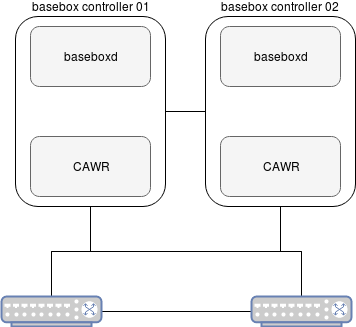
\includegraphics[width=.4\textwidth]{bisdn/basebox}
    \caption{Basebox architecture}
\end{figure}

As the SDN market grows larger and larger in the networking world, new applications and products are developed and improved. Seeing the prevalence of closed source and proprietary solutions for this market, a need for open
products that enable further growth and innovation in cloud DCNs is evident. The main gain in moving from vertically integrated solutions, is the decrease of costs involved, as cheaper solutions can be found in whitebox 
\footnote {whitebox switches are} switches and open sourced networking applications. With this motivation, BISDN developed Basebox, a Linux-powered solution to integrate switches and SDN controllers, allowing for data center 
operators to configure and manage networks using linux commands, removing the need for having to manage several devices with different interfaces and workflows, and adding the capability of running standard networking applications 
on top of the controllers and switches. Basebox also includes the possiblity of running in a failover scenario, by introducing a backup controller for the network, and the possibility of creating a giant switch abstraction, 
by adding another controller, CAWR, and having this manage all the southbound switches.

\par In this chapter we focus on this product, on the first two sections some characteristics of the developed product are described, then we focus on the development of a management API, presenting the required technologies that 
were implemented, and then finally display the results that were obtained in this part of the thesis.

\section {Existing product}

\subsection {baseboxd}
\subsection {CAWR}

\section {Management API}

Due to the capabilities of Basebox of being a SDN controller used in data centers and a mission critical component for the network operators, it needed management capabilities, so that managing and operating infrastructure becomes 
an easier task. As such, the original problem presented was to build an interface extending the original work, so that the network statistics and the information of the topology could be easily displayed. There were several steps
then necessary to understand the problem, and be able to choose the best approach to this problem. The requirements for the proposed system were:

\begin {itemize}
    \item Display the topology information reported by CAWR, including the internal switch links, and the LACP discovered bond interfaces on the servers
    \item Display the port and link statistics for both switches
    \item Design an alerting system, so that network operators can be informed of changes on the network state
    \item Provide some diagnostic capabilities
\end {itemize}

\par The development of the work was the divided on two parts: the first part would be to implement the API needed to export the port statistics from baseboxd and CAWR, including a Graphical User Interface (GUI); and the second 
part was to study the alerting system, that would look into the statistics provided by the controllers, and design some rules so that QoS rules could be applied in the final product. This section describes the technologies needed 
to implement the API for Basebox.

\subsection {Data models}

Data models are abstract concepts that map the properties of entities and organizes their data, also defining how they relate to each other. To create a switch management interface, the entities we want to model are then 
the switches themselves, with attributes like the switch name, and the port counters, and the relationships of the data will allow us to display the links and topology of the network. One of the considerations that were taken into 
account when choosing the data models was the compatibility with standardized data models by the organizational entities like the IETF and the OpenConfig. 
\par The \textit{ NETCONF } network configuration model, which we explore further in \ref{ssec:netconf} also defines a data modelling language known as \textit{ YANG }, which is used in this protocol to model its configuration 
and data,and the remote procedure calls \cite { CITE - rfc 6020 }. By utilizing models defined in this language, the following condition is met: since this is a specific language for configuration and monitoring of networking 
devices, the existing data models will be similar to the ones that should be employed in the development of the management API. YANG data model defines the hierarchy of data between a NETCONF client and server with the objective
of smooth integration with the existing system's infrastructure. 
\par The systems we aim to model with these requirements are then two: the topology between the servers and switches, and the port statistics for each port one the switch. Since there is no data model that would accurately describe
both of them correctly, for the topology we chose the IETF network data model \footnote {https://github.com/YangModels/yang/blob/master/experimental/ietf-extracted-YANG-modules/ietf-network\%402017-12-13.yang}, and the 
OpenConfig interfaces data model \footnote {https://github.com/openconfig/public/tree/1040d11c089c74084c64c234bee3691ec70e8a9f/release/models/interfaces}, which contains the counters for each port.

\subsubsection {Topology}

The topology data model maps a collection of nodes, and the relationships between each node, called a link. This also allows for describing the network in a vertical hierarchy, by displaying relationships between several layers,
which can then be used to display the entire networking stack, for example displaying the physical links between nodes, their connections at layer 2 and layer 3 of the OSI model, and the virtualised relationships that the elements 
could have in a cloud deployement. As the development of the product continues, and more features are added, for example, layer 3 routing, then we require a flexible data model that can be extended to support the new capabilities.

\begin{figure} [!htbp]
    \centering
    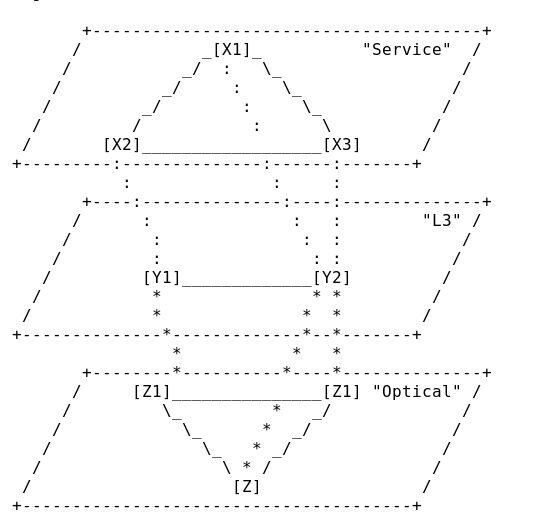
\includegraphics[width=.3\textwidth]{bisdn/network_stack_topologies}
    \caption{Topology hierarchy achievable with this example \cite {CITE - https://www.ietf.org/id/draft-ietf-i2rs-yang-network-topo-20.txt}}
\end{figure}

\par Mapping the data model to the real world data is then adding the two types of information the data model expects: the first one composed of adding the different networks that composed the entire topology, including their
nodes and network types; and then using the previous information to build the links between each of the nodes, using the termination points the model exposes. In the implementation of the management API there was no need to implement 
underlying networks, but the extensibility this provides will be useful in the future.
\par Displaying the topology proved useful for CAWR, which provides the big switch topology, since this controller is directly connected to the underlying switches, and can see the links among these networking devices. The connection
to the bonded interface on the servers can also be monitored, since these can be configured to use LACP messages to report their status. To display the links between the switches, the information that LLDP provides is used, 
and if the controller is extended to be able to use LLDP to the servers, the further information can be filled into this data model, and provide a richer view on the status of each server.

\begin{figure} [h]
    \begin{subfigure}
    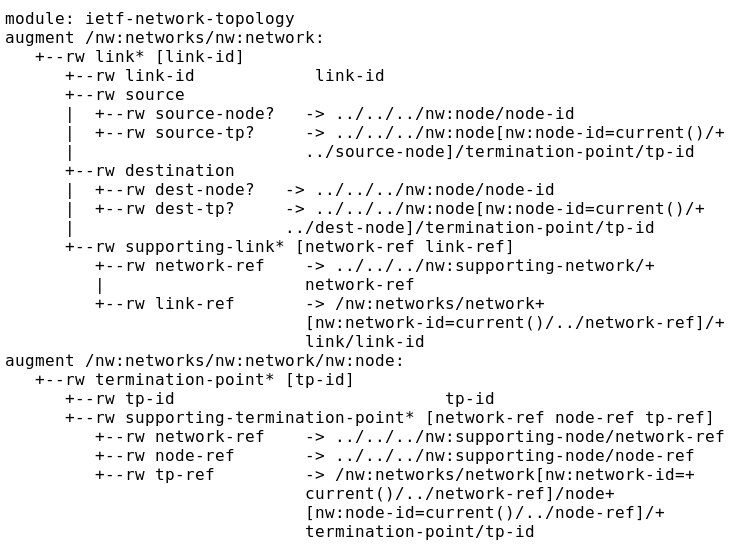
\includegraphics[width=0.5\textwidth]{bisdn/ietf_link}
    \end{subfigure}
    \begin{subfigure}
    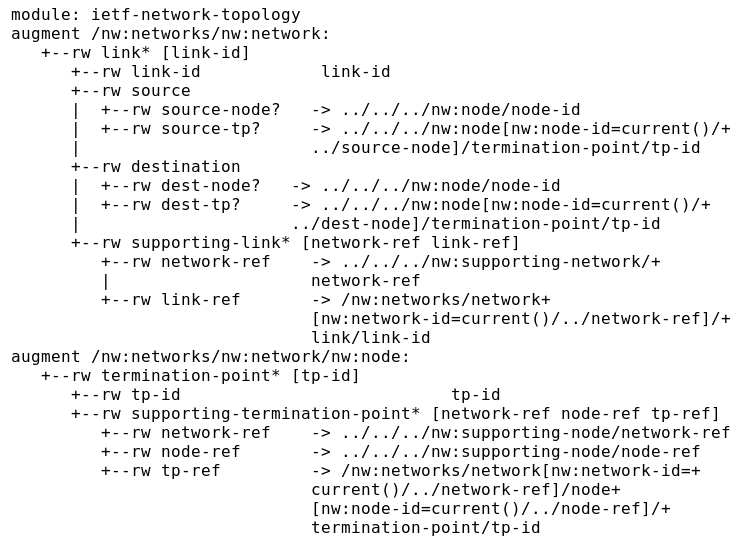
\includegraphics[width=0.5\textwidth]{bisdn/ietf_node}
    \end{subfigure}
\caption{The IETF description for the nodes and links in the draft proposal for network topologies \cite {CITE - https://www.ietf.org/id/draft-ietf-i2rs-yang-network-topo-20.txt} }
\end{figure}

\subsubsection {Port statistics}

\par Modelling the port statistics to build a management interface requires first understanding of the OpenFlow statistics. As previously mentioned, OF switches maintain a set of counters, similar to SNMP, that provide information 
about the state of the ports, group, flow and table stats. The statistics that are exposed from OF are the following:

\begin{table}[]
    \centering
    \caption{OpenFlow port statistics}
    \label{my-label}
    \begin{tabular}{l | l || l | l}
       uint64\_t & rx\_packets     & uint64\_t & tx\_packets;     \\ \hline
       uint64\_t & rx\_bytes;      & uint64\_t & tx\_bytes;       \\ \hline
       uint64\_t & rx\_bytes;      & uint64\_t & tx\_dropped;     \\ \hline
       uint64\_t & rx\_errors;     & uint64\_t & tx\_errors;      \\ \hline
       uint64\_t & rx\_frame\_err; & uint64\_t & tx\_over\_err;   \\ \hline
       uint64\_t & rx\_crc\_err;   &                              \\ \hline
       uint64\_t & collisions;     &                              \\ \hline
       uint32\_t & duration\_sec;  &                              \\ \hline
       uint32\_t & duration\_nsec; &                 
    \end{tabular}
\end{table}

\par The chosen data model should then accurately model the fields that we need to expose, and the data type of counters we wish to measure. In this case, the prevalence of other controllers allows to use the same data models present 
in their implementations. OpenConfig \footnote{http://www.openconfig.net/} maintains a set of vendor neutral data models, written in YANG, allowing network operators to use standardized models for their networking infrastructure.
The entire set of published models can be accessed in their github page \footnote {https://github.com/openconfig/public}.

\subsection {Protocols}

None of the controllers had a clear way of obtaining the statistics apart from manually looking in the terminal and following the logs exposed and waiting for the appropriate output. There needs to be then a controllable, to export
this information and displaying them in a clear way. The solution was to develop a Graphical User Interface (GUI) for easily displaying the live statistics from the server, however there still was the problem of having to 
define the API that build the transport channel between baseboxd and CAWR to the GUI server. In this section we describe the two \textit {Remote Procedure Call (RPC)} systems that were researched, and focus on the advantages which
led to the final decision of implementing gRPC on Basebox.

\subsubsection {NETCONF} \label {ssec:netconf}

Despite it's dominance on network management products, SNMP features some bad characteristics that pose an obstacle for the widespread use in network configuration, and not only network management, like 
\cite {CITE - https://tools.ietf.org/html/rfc3535}: 

\begin {itemize}
    \item Incompleteness of the devices features
    \item SNMP access can sometimes crash systems, or return wrong data
    \item Unavailability of MIB modules, which forces users to use CLI's
    \item Poor performance 
    \item Security is difficult to handle
\end {itemize}

\par The IETF then, in light of this feedback obtained from network operators, started developing a protocol that allowed for the installation, manipulation and deletion of configuration of networking devices called NETCONF, which 
enables devices to expose a full API to their systems. This protocol, based in client/ server communication and is based in the four layers, as can be seen in the following image:

\begin{figure} [!htbp]
    \centering
    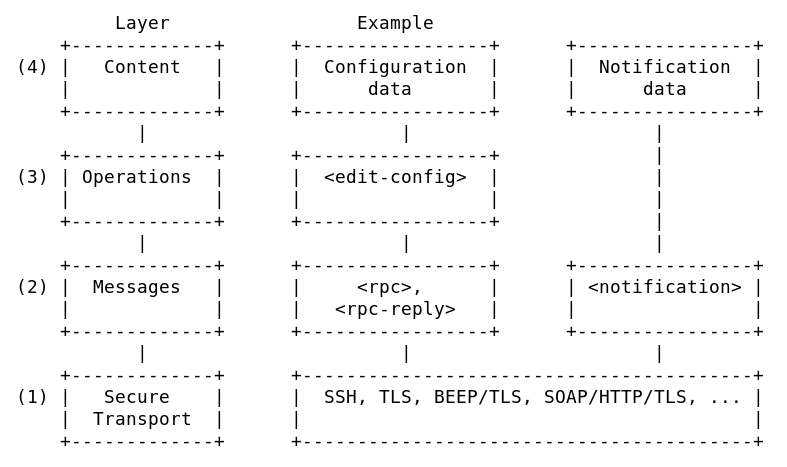
\includegraphics[width=.4\textwidth]{bisdn/netconf}
    \caption{NETCONF protocol layers \cite {CITE - Basebox architecture}}
\end{figure}

\par Data models and operations, covered in detail in the previous section, is related to the Content layer on the image, so this will not be covered in this section. 
\par Configuration of a network device can be complex, and managing separate configurations between device startup and normal operation is a difficult task, but there is occasional need for this capability. NETCONF defines the 
existence of different \textit{datastores} to enable this feature, allowing the network operator to set an initial configuration, used when the device is initialized, and switching to the running datastore when the device is ready
to maintain normal operation. This concept of datastores also enables the creation of a candidate datastore, providing the capability of testing configurations on the network device, checking for any possible errors, while making
sure that there is no impact on the current configuration of the device. After the changes have been tested and validated, a <commit> operation can be used to deploy the new configuration to the running datastore.
\par Another useful feature that is described in the NETCONF protocol, is the possibility of using the rollback-on-error capability. When rolling a new change, and if the system is enabled to support this feature,
NETCONF can detect errors in the changes done to the configurations, and return the system to the previous state that is error free. 
\par The NETCONF API provides several operations to interact with the managed devices to get system information and push new configurations. The set of supported operations in the base NETCONF protocol can be accessed in 
\url{https://tools.ietf.org/html/rfc6241#section-7}. 
\par In regards to the transport layer, NETCONF is able to run on top of several protocols. However, NETCONF requires that a persistent connection is maintained between devices, and this connection should be reliable, and support
transmission failure. In addition, the security should be handled by the transport layer \cite { CITE - https://www.ietf.org/slides/slides-edu-netconf-yang-00.pdf}, providing the guarantee that transactions are done in a 
cryptographically secure channel, between two authenticated hosts. As a results, typical NETCONF implementations are based on SSH or TLS protocols.

\subsubsection {gRPC}  \label {ssec:grpc}

The basic idea behind the RPC system is defining services by setting the interaction between remote systems, allowing for directly calling objects on remote systems. Based in the client/server communications 
pattern, gRPC allows for interactions between different environments, even implemented with different programming languages, all based on the same data structure. This data structure can be serialized using another modelling 
language, called \textit {protobuf}, which will define the data, which is defined as messages, and the services that contain the RPC calls between systems. Since this system is based on the HTTP2 transport layer, we are able to
use the advantages that this protocol provides us.
\par Despite the serialization language used in gRPC is based on protocol buffers, unlike YANG, there are some projects \footnote {https://github.com/openconfig/goyang} that enable the translation between YANG to protofile,
which allows us to use the data models we chose, only adding one extra step to convert the files.
\par Despite both protocols capability of meeting the requirements that were presented to us, the gRPC framework was chosen due to several reasons:

\begin {itemize}
    \item Both frameworks allow us to use the standardized data models currently proposed by the IETF and OpenConfig
    \item NETCONF trades information as XML encoded information, for both the edit and get config operations; while gRPC allows to handle information in a way that’s native to the language implementation of the client/server
    \item The integration with the existing system was easier: since gRPC has implementations for the languages that the controllers are developed on (i.e. C++/ Python), this framework was easier to implement 
        than NETCONF, which would have required integration with third party tools, or a longer development cycle to make sure that the developed applications would met the requirements
\end {itemize}

\section {Results}

 
../doc/chapters/bib.tex
\chapter{Technology Overview} \label{chap:tech} %% chapter 3

\chapter{API Design} \label{chap:api} %% chapter 3

\section {Design}
\section {Implementation}


\chapter{Existing System} \label{chap:system} %% chapter 3


%%\include{chapters/results}
%%\chapter{Conclusion}

\section{Summary of Results}

The main objective for this thesis was building a management system that would integrate with a pre-existing Software-Defined Network controller, exposing information
for network operators to manage and configure their networking infrastructure. With these requirements, we have proposed a management environment that extends a
previously existing system, by adding an interface to baseboxd and CAWR, two SDN controllers composing the Basebox environment, allowing further developments in the 
field of Traffic Engineering with these systems.  Integrating this system, we have designed a Graphical User Interface for interaction with the users, allowing for
simple visualisation of the network's physical topology, and the display of interfaces' statistics, like the packets and bytes received and sent, or the number of 
errors. 

\par We have also proposed an algorithm that allows for monitoring traffic changes in ports, in order to detect elephant flows in the network. Despite not having
used the Basebox system for testing this algorithm, due to differences in the testing environment, we believe that the same algorithm can be used for large flow 
detection in the Basebox stack, by changing the interface for obtaining statistics. We have shown that a simple method can be employed by operators to monitor the
state of their network, and rely on this algorithm to provide them with alarms of port changes.

\section{Future Work}

Despite our conclusion that the main objectives of the thesis were achieved, the large scope of themes that this topic encompasses means that not everything could be 
successfully covered. As for more immediate concerns, the next steps in guaranteeing a stable product would be the expansion  of the GUI to report and configure 
VLANs in each port that is monitored; and support layer 3 functionality, such as visualising next hop neighbours, routing tables, etc. In regards to longer term
goals, continuing the work on monitoring not only the port change, but the actual flow that contributes to the largest changes in ports. This could be expanded 
into a system that analyses the services and applications that contribute the most to the traffic volumes in the network, which can then be further optimized by 
reporting the periodicity of the largest traffic volumes. The aspect of providing a system that can discriminate the traffic by transport protocol is also an 
interesting research topic for improving Quality of Service in Software-Defined Networks.


%% comment next 2 commands if numbered appendices are not used
%\appendix
%\chapter{Appendix}

\section{GUI icons mapping}
\begin{table}[H]
    \centering
    \caption{GUI icons and their meaning}
    \label{tab:gui-mapping}
    \begin{tabular}{l | l}
        \centering
            
\includegraphics[width=.05\textwidth]{bisdn/switch}
        & switch     & \\ \hline 
            
\includegraphics[width=.05\textwidth]{bisdn/host}
        & host     & \\ \hline 
        
\includegraphics[width=.05\textwidth]{bisdn/bond}
        & port     & \\
   \end{tabular}
\end{table}


%%----------------------------------------
%% Final materials
%%----------------------------------------

%% Bibliography
%% Comment the next command if BibTeX file not used
%% bibliography is in ``myrefs.bib''

\PrintBib{Thesus}

%% Index
%% Uncomment next command if index is required
%% don't forget to run ``makeindex thesis'' command
%\PrintIndex

\end{document}
